% 热传导定律
% 热传导|温度梯度|热导率|分子动能

\pentry{梯度 梯度定理\upref{Grad}}
如果气体内各部分的温度不同,从温度较高处向温度较低处,将有热量的传递,这一现象叫做\textbf{热传导(heat conduction)}现象.

\begin{figure}[ht]
\centering
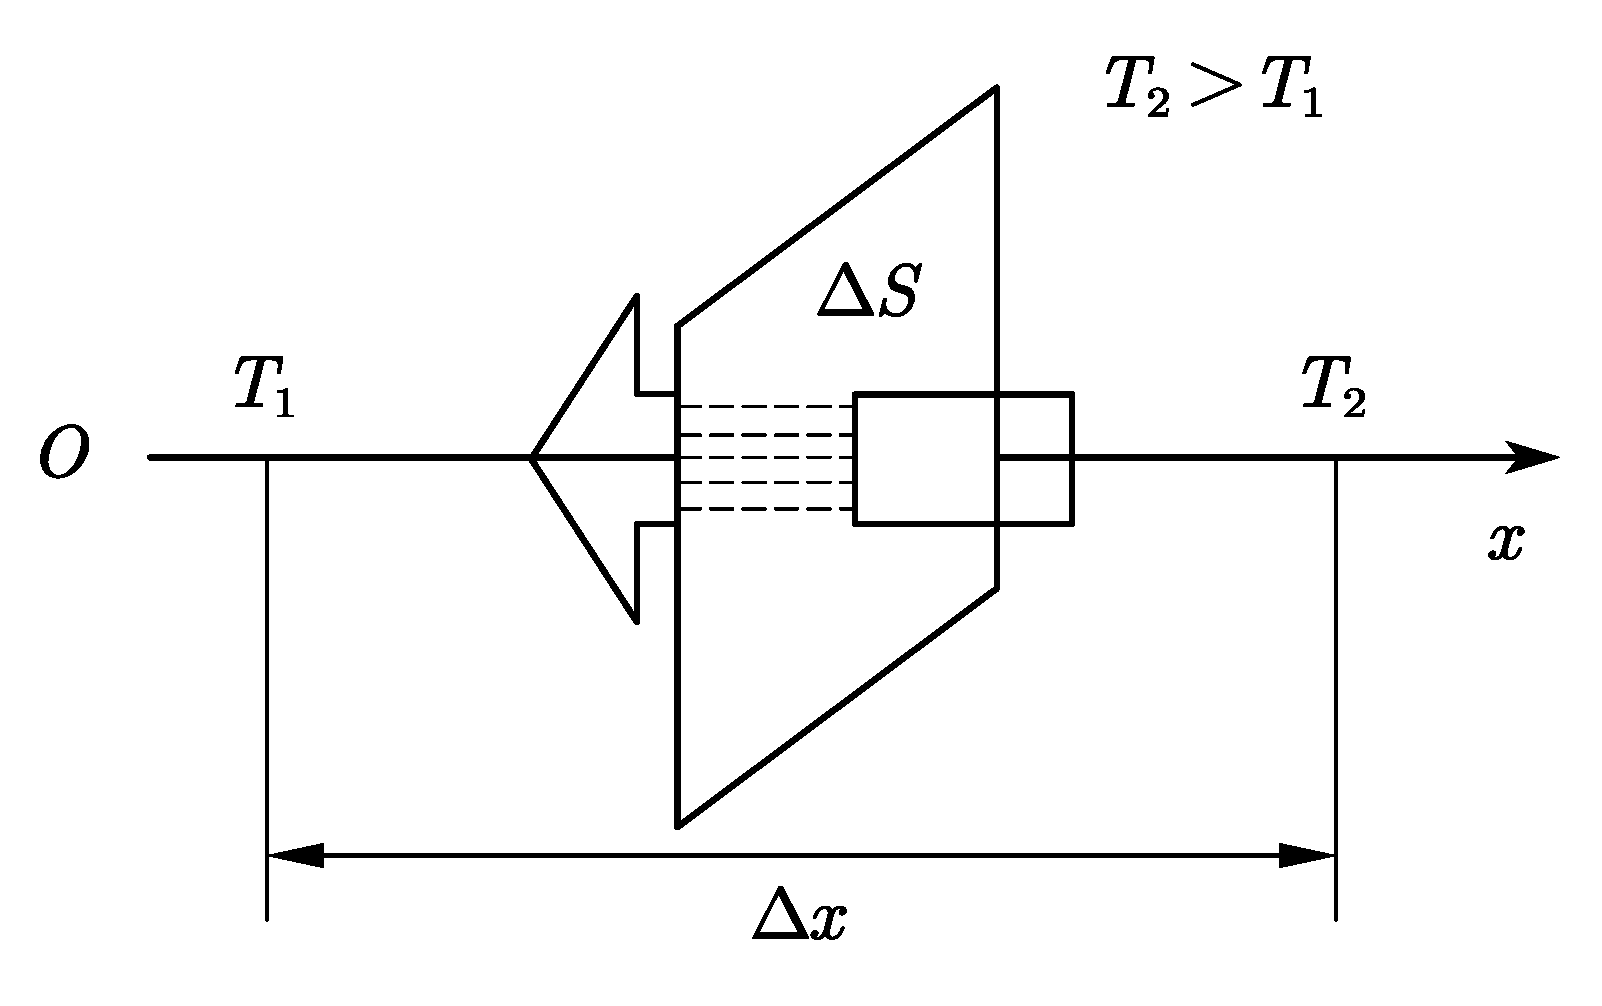
\includegraphics[width=8.5cm]{./figures/Heatco_1.pdf}
\caption{热传导现象} \label{Heatco_fig1}
\end{figure}

如\autoref{Heatco_fig1} 所示,$Ox$轴是气体温度变化最大的方向,在这个方向上气体温度的空间变化率$\mathrm dT/\mathrm dx$,叫做\textbf{温度梯度}.设$\Delta S$为垂直于$Ox $轴的某指定平面的面积.实验证明,在单位时间内,从温度较高的一侧,通过这一平面,向温度较低的一侧所传递的热量,与这一平面所在处的温度梯度成正比,同时也与面积$\Delta S$成正比,即得\textbf{热传导定律}:
\begin{equation}
\frac{\Delta Q}{\Delta t}=-\kappa \frac{\mathrm{d} T}{\mathrm{d} x} \Delta S
\end{equation}
比例系数$\kappa$叫做\textbf{热导率(thermal conductivity)}.式中负号表示热量传递的方向是从高温处传到低温处,和温度梯度的方向是相反的热导率
的单位是$\rm W /(m \cdot K)$.

实验测得,在$0^{\circ} \mathrm{C}$ 时,氢的热导率为$0.168 \mathrm{W} /(\mathrm{m} \cdot \mathrm{K})$,氧力$2.42\times 10^{-1} \mathrm{W} /(\mathrm{m} \cdot \mathrm{K})$, 空气为$\text { 2. } 23 \times 10^{-1} \mathrm{W} /(\mathrm{m} \cdot \mathrm{K})$.在$100^{\circ} \mathrm{C}$ 时,水汽的热导率为$2. 18\times  10{-1}\mathrm{W} /(\mathrm{m} \cdot \mathrm{K})$.显然,气体的热导率都很小,所以,当气体中不存在对流时,气体可用作很好的绝热材料.

在气体动理论中,对气体热传导现象给出这样的解释:在温度较高的热层中,分子平均动能较大;而在温度较低的冷层中,分子平均动能较小.由于冷热两层分子的互相掺和与相互碰撞,从热层到冷层出现热运动能量的净输运.输运的热运动能量,对单原子气体来说,只是分子的平动动能;而对多原子气体来说,还包含转动和振动的能量在内.